\documentclass[red,fullpaper]{ludusofficial}  % Theme: blue, red, green, purple, orange, cyan
                                              % Article type: fullpaper, letter, poster, survey, shortpaper, artpaper

%% Document metadata
\journalname{LUDUS}
\journalsubtitle{International Journal of Game Studies}
\conferencename{LUDUS 2026}
\publicationyear{2026}
% \institution{ludus academik journal}  % This is now set by default in the class file
% \journalurl{https://ludusofficial.site/}  % This is now set by default in the class file
% \articletype{FULL PAPER}  % Set by document class option, or use \articletype{} to customize

%% DOI (optional - leave empty if not assigned yet)
\articledoi{10.1234/ludus.2026.example}

%% Article information
\title{Game Narrative and Player Agency:\\[8pt]A Study in Interactive Storytelling}
\shorttitle{Game Narrative and Player Agency}  % Short title for page headers
\shortauthor{Smith \& Doe}  % Short author names for page headers

\author{%
    \textbf{John Smith}\textsuperscript{1}, \textbf{Jane Doe}\textsuperscript{2}\\[0.2cm]
    \mdseries\small\textsuperscript{1}Department of Game Design, University of Arts, USA\\
    \small\textsuperscript{2}School of Interactive Media, Tech Institute, UK\\
    \small Corresponding: john.smith@university.edu
}

\begin{document}

%% Abstract and keywords must be defined BEFORE \maketitle
\begin{abstract}
This paper examines the relationship between narrative structures and player agency in digital games. We analyze how interactive storytelling techniques create unique aesthetic experiences that distinguish games from traditional narrative media. Through case studies of contemporary games, we identify three key dimensions of player agency: operational interaction, choice-based interaction, and emergent interaction. Our findings reveal that successful game narratives balance authorial control with player freedom, creating what we term ``collaborative storytelling.'' This research contributes to game studies theory and provides practical insights for game designers seeking to enhance narrative engagement.
\end{abstract}

\keywords{game narrative; player agency; interactive storytelling; game design; procedural rhetoric; emergent gameplay}

%% Maketitle creates full-width header with abstract and keywords, then starts two-column layout
\maketitle

%% From here, content is in two columns
\section{Introduction}

Digital games represent a unique form of narrative media, distinguished by their interactive nature. Unlike traditional storytelling forms such as literature or film, games position players not as passive consumers but as active participants in the narrative construction process\footnote{This participatory dimension fundamentally transforms the relationship between story and audience.}. This transformation has profound implications for how we understand narrative theory and practice in the digital age.

Recent scholarship in game studies has increasingly focused on the mechanics of interactive storytelling~\cite{murray1997,jenkins2004}. However, there remains significant debate about the optimal balance between narrative structure and player freedom. Some designers prioritize tight narrative control to ensure coherent storytelling, while others embrace emergent narratives that arise from player interaction with game systems.

\subsection{Research Context}

The evolution of game narrative has progressed from simple text-based adventures to complex multi-threaded story systems. Early games like \textit{Adventure} (1976) and \textit{Zork} (1980) relied primarily on textual description, with players typing commands to navigate virtual worlds. As graphical capabilities improved, games began incorporating cinematic techniques, leading to more sophisticated narrative presentations.

Contemporary games demonstrate diverse approaches to storytelling. Narrative-driven games such as \textit{The Last of Us} series achieve cinematic depth, while experimental titles like \textit{Journey} (2012) explore more abstract narrative forms. This diversity suggests that interactive narrative remains an evolving art form with unexplored potential.

\subsection{Theoretical Framework}

This study builds on three foundational concepts: Janet Murray's notion of the ``Holodeck''~\cite{murray1997}, emphasizing the immersive and participatory qualities of digital media; Henry Jenkins's theory of ``environmental storytelling''~\cite{jenkins2004}, which highlights the role of spatial design in narrative construction; and Ian Bogost's concept of ``procedural rhetoric''~\cite{bogost2007}, revealing how game mechanics themselves convey meaning.

\subsubsection{Dimensions of Player Agency}

Player agency constitutes the core characteristic of game narratives. We identify three distinct dimensions: \textit{operational agency} refers to moment-to-moment control over avatar actions; \textit{choice agency} involves decision-making at narrative branch points; and \textit{emergent agency} describes unpredictable narrative outcomes arising from complex system interactions.

\section{Methodology}

This research employs qualitative methods combining textual analysis and case studies. We selected ten representative narrative-driven games spanning different genres and design philosophies, including \textit{The Last of Us Part II}, \textit{Detroit: Become Human}, \textit{The Legend of Zelda: Breath of the Wild}, and \textit{Death Stranding}.

Our analysis proceeded in three phases: first, extensive gameplay to identify key narrative structures and interaction patterns; second, systematic analysis of narrative mechanisms, character development, and thematic expression; finally, theoretical interpretation connecting findings to existing game narrative theory.

\begin{figure}[h!]
    \centering
    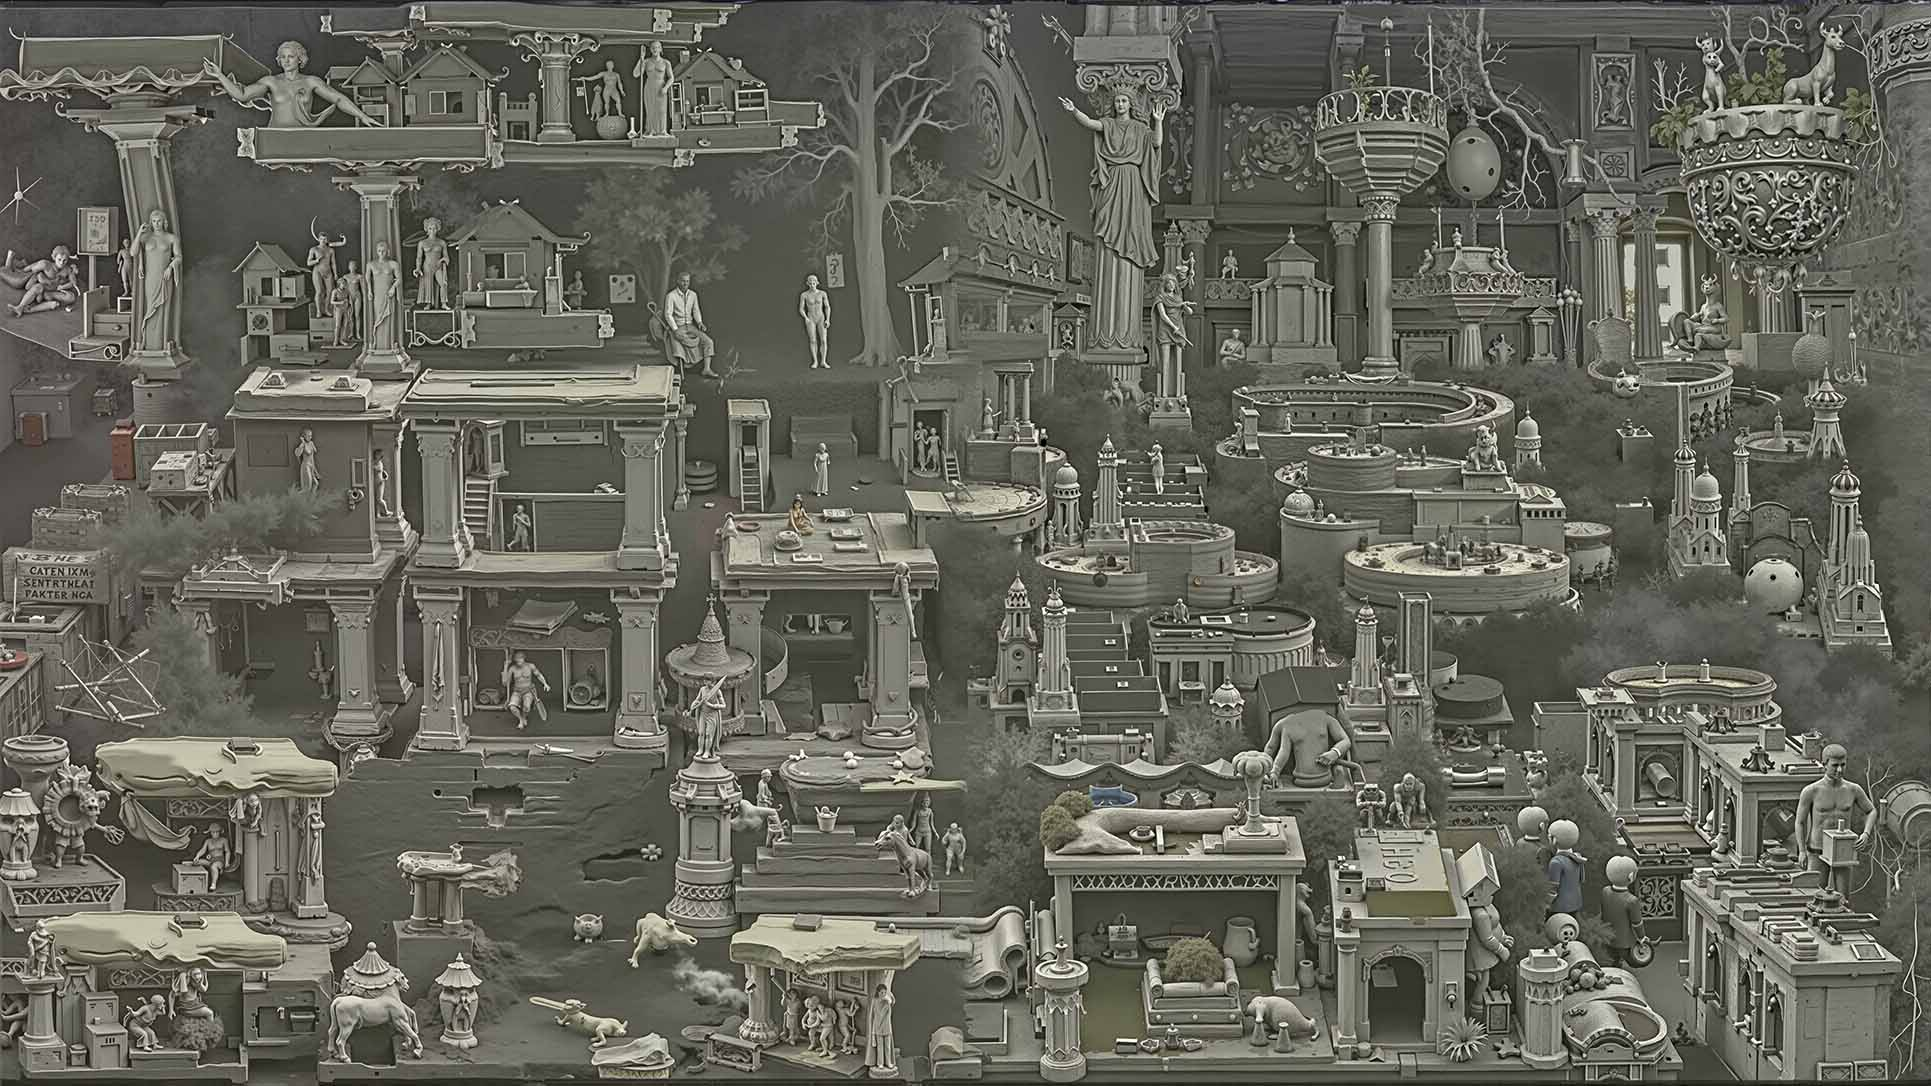
\includegraphics[width=\columnwidth]{testImg.jpg}
    \caption{Conceptual model of interactive narrative dimensions}
    \label{fig:narrative-model}
\end{figure}

\section{Findings}

Analysis of case study games reveals several core characteristics of digital game narratives.

\subsection{Procedural Narrative}

Game narratives are not fixed predetermined texts but dynamically generated through procedural logic. This procedural characteristic means each player's experience potentially differs, transforming narrative from singular linear sequences into spaces of narrative possibility. In \textit{Detroit: Become Human}, for instance, player choices lead to dozens of distinct endings.

\subsection{Player Agency}

In game narratives, players transcend witnessing to become co-creators of story. Through character control, decision-making, and environmental exploration, players actively participate in narrative construction. This agency grants players unprecedented narrative subjectivity while challenging game designers to accommodate diverse playstyles.

\subsection{Emergent Experience}

Complex game systems often produce narrative effects designers never anticipated. This emergence arises from mechanical interplay and creative gameplay approaches. In \textit{The Legend of Zelda: Breath of the Wild}, players combine different mechanics to create unique problem-solving methods and combat strategies, generating personalized narrative experiences.

\begin{table}[h!]
\centering
\caption{Narrative characteristics by game type}
\label{tab:game-types}
\begin{tabular}{lcc}
\hline
\textbf{Game Type} & \textbf{Agency Level} & \textbf{Narrative Depth} \\
\hline
Linear narrative & Low & High \\
Open world & High & Medium \\
Procedural generation & High & Low \\
\hline
\end{tabular}
\end{table}

\section{Discussion}

This research reveals the unique aesthetic characteristics of digital game narratives, which contrast sharply with traditional narrative media. Game narrative value lies not only in telling compelling stories but in creating distinctive aesthetic experiences—experiences combining interaction, immersion, and emergence.

However, game narrative development also faces significant challenges. How can designers maintain narrative coherence while granting sufficient player freedom? How can they balance gameplay and narrative? These questions require further exploration. Future research directions include: investigating new narrative technologies such as AI-driven dynamic storytelling; examining narrative experience differences across cultural backgrounds; and studying cross-media adaptation of game narratives.

\section{Conclusion}

Digital games, as an emerging narrative medium, demonstrate distinctive artistic value. Their interactive, procedural, and emergent characteristics collectively shape aesthetic experiences unlike those of traditional media. Through systematic analysis of game narrative mechanisms, this research provides new theoretical perspectives for game studies while offering practical insights for game design practice.

As technology advances and creative concepts deepen, we have reason to believe digital games will open ever-broader territories in the narrative arts, bringing increasingly rich and diverse experiences to human cultural life.

\begin{acknowledgments}
This research was supported by the Game Studies Research Initiative. We thank the anonymous reviewers for their valuable feedback and suggestions.
\end{acknowledgments}

%% References using BibTeX
%% Make sure to compile with: pdflatex -> bibtex -> pdflatex -> pdflatex
\bibliographystyle{plain}
\bibliography{references}

\end{document}
